\documentclass[tikz,border=4pt]{standalone}
\usepackage{ctex}
\usepackage{amsmath}
\usepackage{pgfplots}
\pgfplotsset{compat=1.18}
\begin{document}
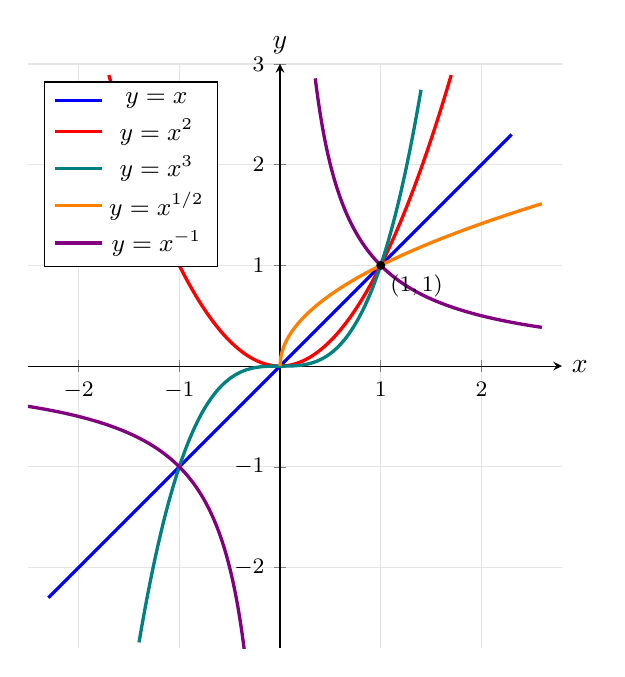
\begin{tikzpicture}
\begin{axis}[
    axis lines=middle,
    xmin=-2.5, xmax=2.8,
    ymin=-2.8, ymax=3.0,
    width=10cm, height=9cm,
    xlabel={$x$}, ylabel={$y$},
    xlabel style={right}, ylabel style={above},
    samples=300,
    grid=both,
    grid style={gray!20},
    legend pos=north west,
    legend style={font=\small},
    axis equal image,
    tick label style={font=\footnotesize},
    restrict y to domain=-3:3,
]
\addplot[blue, very thick, domain=-2.3:2.3] {x};
\addlegendentry{$y=x$}
\addplot[red, very thick, domain=-1.7:1.7] {x^2};
\addlegendentry{$y=x^2$}
\addplot[teal, very thick, domain=-1.4:1.4] {x^3};
\addlegendentry{$y=x^3$}
\addplot[orange, very thick, domain=0:2.6] {sqrt(x)};
\addlegendentry{$y=x^{1/2}$}
\addplot[violet, very thick, domain=0.35:2.6] {1/x};
\addplot[violet, very thick, domain=-2.6:-0.35] {1/x};
\addlegendentry{$y=x^{-1}$}
\addplot[only marks, mark=*, mark size=1.4pt, black] coordinates {(1,1)};
\node[below right, font=\footnotesize] at (axis cs:1,1) {$(1,1)$};
\end{axis}
\end{tikzpicture}
\end{document}
